\documentclass{standalone}

\usepackage{libertinus}
\usepackage[T1]{fontenc}
\renewcommand*\familydefault{\sfdefault}

\usepackage{DejaVuSansMono}

\usepackage{tikz}
\usetikzlibrary{decorations.pathmorphing, decorations.pathreplacing, decorations.shapes}
\tikzset{every path/.style={semithick}}

\begin{document}
  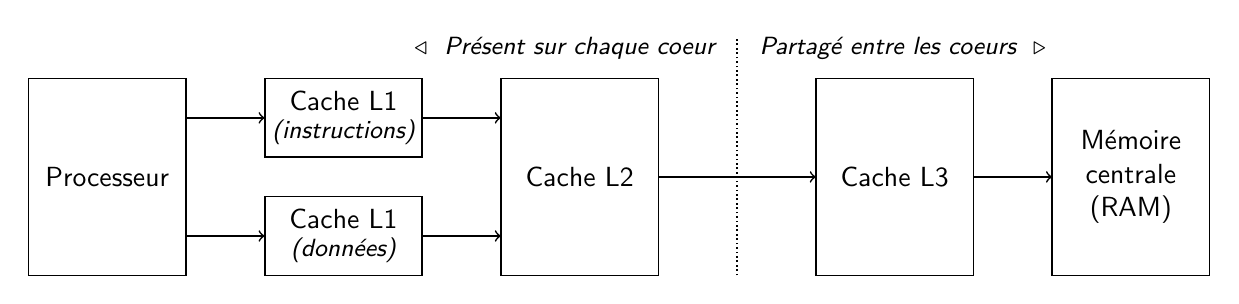
\begin{tikzpicture}
    \draw (0,0) rectangle node[align=center] {Processeur} ++(2,2.5);

    \draw (3,1.5) rectangle node[align=center] {Cache L1 \\[-2pt] \small\it (instructions)} ++(2,1);
    \draw (3,0) rectangle node[align=center] {Cache L1 \\[-2pt] \small\it (données)} ++(2,1);

    \draw (6,0) rectangle node[align=center] {Cache L2} ++(2,2.5);

    \draw (10,0) rectangle node[align=center] {Cache L3} ++(2,2.5);

    \draw (13,0) rectangle node[align=center] {Mémoire \\ centrale \\ (RAM)} ++(2,2.5);

    \draw[densely dotted] (9,0) -- ++(0,3)
      node[below left, text depth=0.2ex, yshift=1ex, xshift=-1ex] {\small\it $\triangleleft$~~Présent sur chaque coeur}
      node[below right, text depth=0.2ex, yshift=1ex, xshift=1ex] {\small\it Partagé entre les coeurs~~$\triangleright$};

    \draw[->] (2,0.5) -- ++(1,0);
    \draw[->] (2,2) -- ++(1,0);

    \draw[->] (5,0.5) -- ++(1,0);
    \draw[->] (5,2) -- ++(1,0);

    \draw[->] (8,1.25) -- ++(2,0);
    \draw[->] (12,1.25) -- ++(1,0);
  \end{tikzpicture}
\end{document}
